\documentclass[border=2pt]{standalone}
\usepackage{tikz}
\usetikzlibrary{arrows.meta,positioning}
\begin{document}
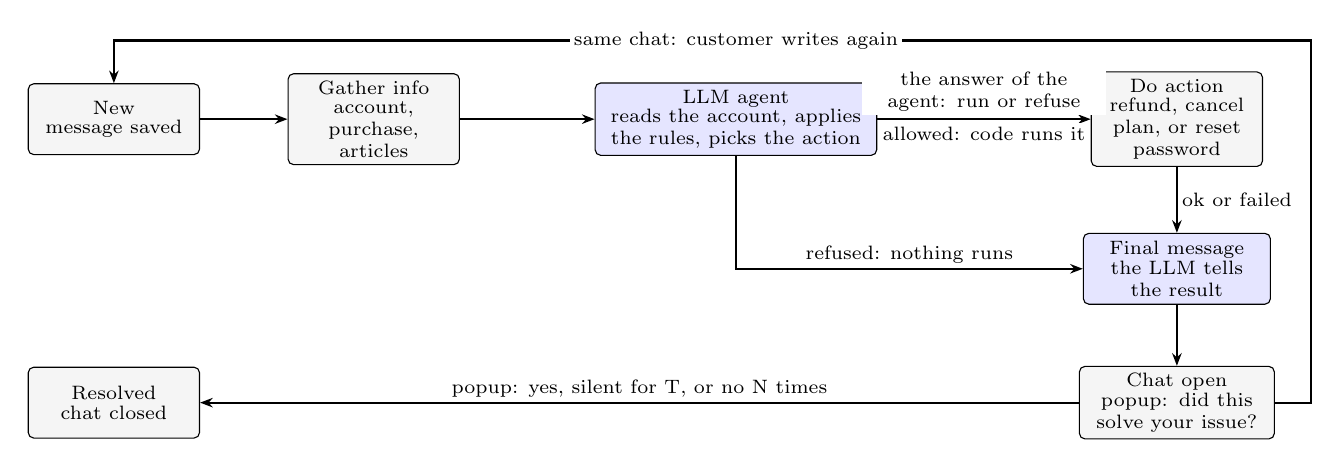
\begin{tikzpicture}[
  every node/.style={font=\scriptsize},
  st/.style={draw, rounded corners=2pt, minimum height=9mm, text width=20mm, align=center, inner sep=2.5pt},
  fx/.style={st, fill=gray!8},
  md/.style={st, fill=blue!10},
  rl/.style={st, fill=green!14},
  ar/.style={-{Stealth[length=1.6mm]}, thick},
  lb/.style={font=\scriptsize, inner sep=1.5pt, fill=white, text width=16mm, align=center},
  lw/.style={font=\scriptsize, inner sep=1.5pt, fill=white}]
  \node[fx] (new) at (0,0) {New\\[-1pt]{\scriptsize message saved}};
  \node[fx] (gat) at (3.3,0) {Gather info\\[-1pt]{\scriptsize account, purchase, articles}};
  \node[md, text width=34mm] (age) at (7.9,0) {LLM agent\\[-1pt]{\scriptsize reads the account, applies the rules, picks the action}};
  \node[fx] (act) at (13.5,0) {Do action\\[-1pt]{\scriptsize refund, cancel plan, or reset password}};
  \node[md, text width=22mm] (fin) at (13.5,-1.9) {Final message\\[-1pt]{\scriptsize the LLM tells the result}};
  \node[fx, text width=23mm] (cha) at (13.5,-3.6) {Chat open\\[-1pt]{\scriptsize popup: did this solve your issue?}};
  \node[fx] (res) at (0,-3.6) {Resolved\\[-1pt]{\scriptsize chat closed}};

  \draw[ar] (new) -- (gat);
  \draw[ar] (gat) -- (age);
  \draw[ar] (age) -- node[lb, above=1pt, text width=30mm]{the answer of the agent: run or refuse} node[lw, below=1pt]{allowed: code runs it} (act);
  \draw[ar] (act) -- node[lw, right]{ok or failed} (fin);
  \draw[ar] (age.south) |- node[lw, above, pos=0.75]{refused: nothing runs} (fin.west);
  \draw[ar] (fin) -- (cha);
  \draw[ar] (cha.west) -- node[lw, above]{popup: yes, silent for T, or no N times} (res.east);
  \draw[ar] (cha.east) -- (15.2,-3.6) -- (15.2,1.0) -- (new.north |- 0,1.0) -- (new.north);
  \node[lw] at (7.9,1.0) {same chat: customer writes again};
\end{tikzpicture}
\end{document}
